\documentclass[conference]{IEEEtran}
\IEEEoverridecommandlockouts
% The preceding line is only needed to identify funding in the first footnote. If that is unneeded, please comment it out.
\usepackage{cite}
\usepackage{amsmath,amssymb,amsfonts}
\usepackage{algorithmic}
\usepackage{graphicx}
\usepackage{textcomp}
\usepackage{xcolor}
\usepackage{verbatim}
%KHOA BEGIN
\usepackage{multirow}
\usepackage{array}
%KHOA END

\ifCLASSOPTIONcompsoc
    \usepackage[caption=false, font=normalsize, labelfont=sf, textfont=sf]{subfig}
\else
\usepackage[caption=false, font=footnotesize]{subfig}

\def\BibTeX{{\rm B\kern-.05em{\sc i\kern-.025em b}\kern-.08em
    T\kern-.1667em\lower.7ex\hbox{E}\kern-.125emX}}
\begin{document}

\title{Strategies to meet the configured repetitions in URLLC Uplink Grant-Free transmission\\
%{\footnotesize \textsuperscript{*}Note: Sub-titles are not captured in Xplore and
%should not be used}
%\thanks{Identify applicable funding agency here. If none, delete this.}
}

\author{\IEEEauthorblockN{Trung-Kien Le$^{\dagger}$, Umer Salim$^{\star}$, Florian Kaltenberger$^{\dagger}$}
\IEEEauthorblockA{$^{\dagger}$EURECOM, Sophia-Antipolis, France \\
%\textit{name of organization (of Aff.)}\\
$^{\star}$TCL Mobile, Sophia-Antipolis, France \\
Trung-Kien.Le@eurecom.fr}
%\and
%\IEEEauthorblockN{Umer Salim}
%\IEEEauthorblockA{\textit{TCL Communication} \\
%\textit{name of organization (of Aff.)}\\
%Paris, France \\
%Emails: umer.salim@tcl.com}
%\and
%\IEEEauthorblockN{3\textsuperscript{rd} Given Name Surname}
%\IEEEauthorblockA{\textit{dept. name of organization (of Aff.)} \\
%\textit{name of organization (of Aff.)}\\
%City, Country \\
%email address}
%\and
%\IEEEauthorblockN{4\textsuperscript{th} Given Name Surname}
%\IEEEauthorblockA{\textit{dept. name of organization (of Aff.)} \\
%\textit{name of organization (of Aff.)}\\
%City, Country \\
%email address}
%\and
%\IEEEauthorblockN{5\textsuperscript{th} Given Name Surname}
%\IEEEauthorblockA{\textit{dept. name of organization (of Aff.)} \\
%\textit{name of organization (of Aff.)}\\
%City, Country \\
%email address}
%\and
%\IEEEauthorblockN{6\textsuperscript{th} Given Name Surname}
%\IEEEauthorblockA{\textit{dept. name of organization (of Aff.)} \\
%\textit{name of organization (of Aff.)}\\
%City, Country \\
%email address}
}

\maketitle

\begin{abstract}
In Ultra-Reliable Low-Latency Communication (URLLC), the user (UE) can be configured to transmit in grant-free/configured-grant (GF/CG) resources for  uplink (UL) transmission that does not require the UE to transmit scheduling request (SR) and receive UL grant to reduce latency. In addition, the UE is also configured to transmit automatically a specific number of repetitions. However, these repetitions are only allowed to carry out in an interval with period $P$ to avoid identity (ID) confusion in a Hybrid automatic repeat request (HARQ) process. Thereby, there is a chance that the UE cannot transmit all repetitions as configured if data arrives late and it leads to a drop of reliability. Two approaches are proposed in this paper to cope with this problem. This first approach requires an usage of the explicit Hybrid automatic repeat request (HARQ) feedback structure and the second one is related to an additional SR transmitted by the UE. The numerical results show the benefit of these two methods in increasing system performance in case of less configured repetitions made when they help the system to avoid or reduce packet loss due to Demodulation Reference Signal (DMRS) miss-detection.
\end{abstract}

\begin{IEEEkeywords}
5G, URLLC, grant-free repetitions, uplink scheduling scheme, explicit HARQ feedback, scheduling request
\end{IEEEkeywords}

\section{Introduction} \label{I}
The advent of new applications such as remote surgery, vehicle-to-everything communication, etc. with high demands of latency and reliability requires that 5G supports URLLC. The strict requirements of URLLC are given in \cite{b6}: ``A general URLLC reliability requirement for one transmission of a packet is 10\textsuperscript{-5} for 32 bytes with a user plane latency of 1 ms''. These requirements continue to rise in the recent meetings of the 3rd Generation Partnership  Project  (3GPP): ``Higher reliability (up to 10\textsuperscript{-6}), higher availability, short latency in the order of 0.5 to 1 ms, depending on the use cases (factory automation, transport industry and electrical power distribution)''\cite{b8}.

\subsection{Techniques accepted in 3GPP Release 15}\label{IAA}
In order to facilitate the implementation of URLLC, 3GPP made three important decisions about physical layer design.

One of the aspects is a permission to use larger subcarrier spacings (SCS). In 5G, SCS is allowed to have a value up to 240 kHz instead of an unique value of 15 kHz as in LTE \cite{ad2}. The next aspect is about mini-slot based transmission that allows a UE to be scheduled in a period of one or several symbols rather than a whole slot \cite{ad3}. These two decisions bring down time alignment of arriving packets.

The third aspect is related to the UL transmission in GF region to lessen time consumption of SR and UL grant\cite{ad4}.

\subsection{Repetition problem in URLLC GF UL transmission}\label{IBB}
As mentioned in Section \ref{IAA}, in UL transmission, the base station (called gNB) can configure a set of GF resources to one or more UEs with a periodicity defined by parameters in Radio Resource Control (RRC) from higher layer. When a UE is configured to transmit in GF resources, it can transmit data immediately instead of sending SR and waiting for UL grant as grant-based (GB) transmission.

To further reduce latency as well as increase reliability of the transmission, the URLLC UEs transmitting in the GF regions are also configured to transmit automatically a number of repetitions (called $K$ repetitions with $K \in \{1, 2, 4, 8\}$ \cite{ad5}) defined by a parameter repK from higher layer instead of waiting an UL grant to reschedule data if necessary after each repetition. Nevertheless, the UEs are only permitted to carry out the repetitions in one HARQ process with a periodicity $P$ as shown in Fig.~\ref{fig1} (a set of allowed periodicities $P$ are defined in \cite{ad5}). Thereby, the UEs stop to do the repetitions at the boundary of a HARQ process even if they still do not reach the configured number of repetitions. In Fig.~\ref{fig1}, an interval $P$ contains 4 GF occasions, the UE is configured to do 4 repetitions. In the first period, data comes before all the 4 GF occasions so the UE is able to do 4 repetitions for the first packet as configured. However, when data comes in the second period, there are only 3 GF occasions left in that period. This means that the UE only can carry out 3 repetitions that are less than the configured number. Similarly, in the fourth period, the UE only can transmit the packet 2 times. 
\begin{figure}[htbp]
\centerline{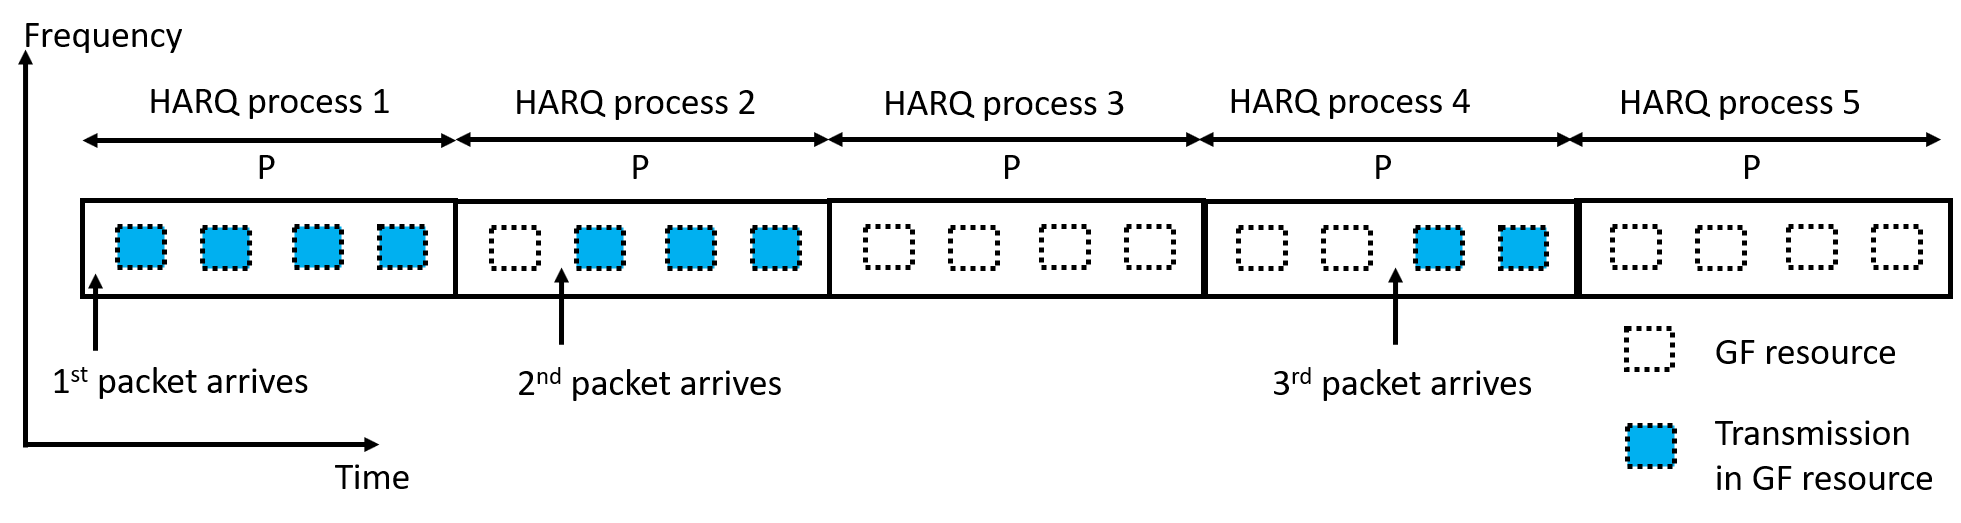
\includegraphics[scale=0.25]{fig1.png}}
\caption{Less than K repetitions in GF UL transmission.}
\label{fig1}
\vspace{-2mm}
\end{figure}

This constraint is to help the gNB avoid a confusion in HARQ IDs of different HARQ processes that preventing its from recognizing the first repetition to do soft combining or determining the UE IDs to send an UL grant. However, this constraint also makes the system face a degradation of UL transmission's performance due to a smaller number of repetitions that is catastrophic to the URLLC UEs with high reliability requirement. It also impacts latency when the gNB cannot decode the packet because the configured number of repetitions are not transmitted, it must schedule a retransmission by an UL grant and the UE only carries out more retransmissions after receiving this UL grant.

\subsection{Prior art}\label{ICC}
In 3GPP Release 15, an option for the UE is to wait until the next HARQ process to transmit the whole K repetitions if it cannot make K repetitions as configured in the current process because data comes late. This method leads to huge latency and might not suitable for URLLC.

In \cite{b1} and \cite{b2}, the UE does not stop at the boundary of a period $P$ if the configured number of repetions have not been reached. The UE is allowed to continue to transmit the repetitions across the boundary and only stops after transmitting all K repetitions. To avoid a confusion of HARQ ID as mentioned in Section \ref{IBB}, a new mechanism needs to be defined to communicate explicitly HARQ ID from the UE to the gNB and results in big overhead and effort in standardization.  

Multiple configurations in GF region are proposed in \cite{b3} and \cite{b4}. A UE is configured with configurations having different starting time offsets so it can choose the nearest configuration to start a transmission without having to wait long time until the next period and guarantee the number of repetitions. However, this method causes big overhead from downlink control information (DCI) used to configure different configurations to the UEs. Resource consumption is another concern, if the configurations are configured separately without any overlap. 

\cite{b5} and \cite{b7} propose to use shared resource for URLLC repetitions to improve resource utilization. However, they do not count a constraint that the UE cannot do repetitions crossing the border of a period. If this constraint is not solved, it might lead to a number of repetitions smaller than the  number configured and transmission reliability is degraded.

In this work, two methods are presented to enhance the performance of URLLC UL GF transmission in case the UE cannot make K repetitions as configured. The first method described in Section \ref{II} applies an explicit HARQ feedback structure to the transmisisons with less than K repetitions. The second method in Section \ref{III} asks the UEs with less than K repetition to transmit a SR in parallel with data packet. These two methods guarantee a retransmission in case of DMRS miss-detection due to a smaller number of repetitions. Section \ref{IV} shows numerical results and performance evaluation. Finally, Section \ref{V} provides the concluding remarks.

\section{Improving reliability-latency by flexibly moving to explicit HARQ Feedback structure}\label{II}

\subsection{Operation of explicit HARQ feedback structure}\label{IIAA}

The HARQ structure in UL GF transmission is timer-based. This means that there is no explicit acknowledgement (ACK) feedback sent from the gNB to the UE if data is decoded correctly. Instead, the UE uses a timer. If it does not receive an UL grant to schedule a retransmission at the end of time configured in the timer, the transmission is considered as successful. This structure has a drawback because the UE cannot differentiate between a successful transmission and a miss-detection when the gNB cannot decode DMRS to identify the UE and transmits UL grant. Therefore, in case of miss-detection, the UE does not receive any signal from the gNB, it assumes a successful transmission and drops data in buffer. This behavior impacts reliability of a transmission and becomes more severe in less-than-K-repetitions situation. Once the UE is not able to carry the configured number of repetitions, the QoS of transmission is badly affected and there is a higher probability that the gNB cannot decode DMRS sequence. It leads to a degradation of URLLC transmission due to packet dropped by the UE. To handle the issue with GF transmissions with less than K repetitions, we propose to use explicit HARQ feedback from the gNB. 

An UL transmission results in three scenarios: one for correct decoding and two scenarios for incorrect decoding. In explicit HARQ feedback structure, the UE's behavior in each scenario will be analyzed as follows. 

The first scenario is about correct data decoding. The gNB tries to combine all the repetitions of a TB to facilitate data decoding, and the number of these repetitions can be less than K as per the previous discussion. For a normal operation, the gNB is capable of identifying the repetitions concerning a specific TB. Thus, whenever the gNB is able to correctly decode a TB, and it sees that it was sent with less than K repetitions, it will send an explicit ACK for this TB to the transmitting UE.

The second scenario is about a failure of data decoding with a successful UE identification. When the UE transmits less than K repetitions, it is possible that the data decoding is not successful but the gNB is able to identify the UE transmitting the TB with less than K repetitions through identification of UE specific DMRS sequence which it was configured with as part of CG configuration. In this case, the gNB will reschedule a retransmission of the previously transmitted TB. 

The third scenario is related to UE identification failure. It is where the proposed explicit feedback becomes pivotal. The bad quality of received data may lead to a situation when the gNB is unable to identify the transmitting UE. This situation is the most damaging for the URLLC UEs/applications due to their tight constraints on latency and reliability. With a timer-based HARQ structure, which is currently used for URLLC transmissions in 3GPP Release 15, this situation leads to different understanding at the gNB and at the UE. The gNB, being unable to identify the UE, cannot schedule the re-transmission. The UE, upon receiving no UL grant for re-transmission, considers the packet successfully decoded at the gNB and discards the buffer upon the expiry of HARQ timer.

Although the situation when the gNB cannot identify the UE may be caused by a number of reasons such as the very bad channel conditions, large amount of interference or insufficient number of actual repetitions, the configuration parameters of CG transmission, in particular MCS and the number of repetitions K, are designed to combat most of these adverse effects. On the other hand, if the configured number of repetitions cannot be made, this brings the CG operation point to a lower QoS target than the desired operating point.

In the proposed technique, whenever the UE transmits less than K repetitions, the TB in question is supposed to operate with explicit HARQ based feedback. In general, the gNB can identify transmissions with less than K repetitions thanks to DMRS detection and CG window boundary knowledge. When the gNB fails to identify the transmitting UE and sends no ACK or UL grant to this UE, the UE upon expiry of configured HARQ timer re-transmits automatically the TB. 

The retransmission timing and resources can be configured as part of the explicit HARQ feedback configuration. One suitable option is to retransmit in the closest CG periodic window after the expiry of HARQ feedback timer. The HARQ feedback timer should include the time for the gNB to decode the data and find the suitable occasion for potential DL transmission of HARQ ACK or UL grant.

\subsection{Design of explicit HARQ feedback}\label{IIBB}

In the proposed strategy, the UEs are allowed to request explicit HARQ feedback for certain TBs. Thus, a design for the explicit HARQ feedback in general may be needed. One strategy can be to define a channel where HARQ ACK can be transmitted. This can be similar to Physical HARQ Indicator Channel (PHICH) as specified in 4G LTE but this requires a lot of specification effort and high resource overhead. The rationale is that in typical operation mode, the UEs will not request explicit HARQ feedback to reduce overhead and only in exceptional cases it will be required. 

With this in view, the proposal is to use the UL grant (which is DCI) as an explicit HARQ feedback. This DCI can be sent with UE specific configured scheduling-radio network temporary identifier (CS-RNTI) which is used with configured GB transmissions. If the gNB is able to successfully decode the data, it sends DCI to this UE with the same HARQ process number (HARQ ID) as of the successfully received TB. To avoid any confusion between DCI used as feedback and DCI used as UL grant, new data indicator (NDI) field can be set to 0. Further, some of the fields in the DCI such as the time and frequency resource assignment fields are set to 0 to help the UE differentiate two types of DCI .

\section{Improving reliability-latency by flexibly transmitting an additional Scheduling Request }\label{III}

In this section, another scheme is proposed to deal with the problem of less-than-K repetitions. In this scheme to improve the reliability of UL GF transmissions, whenever the UE transmits less than the configured number of repetitions for a TB, it sends SR to the gNB, in parallel to transmission of TB with less than K repetitions. This SR provides a sort of diversity mechanism in parallel to the transmission of the TB.

3GPP Release 15 does not allow transmission of Physical uplink control channel (PUCCH) and Physical uplink shared channel (PUSCH) simultaneously. The UE transmits UCI encoding SR, HARQ feedback, etc on PUCCH. Therefore, the UE multiplexes UCI and PUSCH if it wants to transmit uplink control information (UCI) while sending PUSCH. This strategy allows the UE to transmit SR in case of less than K repetitions. However, in UCI and PUSCH  multiplexing, if the gNB cannot detect DMRS of PUSCH due to bad channel, there is high probability that the gNB also cannot decode UCI (SR) to find the UE ID. Thus, multiplexing strategy might not enhance the performance of UE ID detection. For this reason, SR should be configured to be transmitted on the configured PUCCH resources. The gNB upon receiving PUCCH and PUSCH from the same UE will understand that the SR in PUCCH is for the same TB sent in PUSCH for the UE that is only able to make less than K repetitions.

Table~\ref{tab1} shows in tabular format the UE and gNB actions for strategy of SR transmission in parallel to TB transmission. 

\begin{table*}[htbp]
\caption{SR Transmission with TB and Actions for the gNB and the UE}
\begin{center}
\begin{tabular}{|p{1.5em}|p{10em}|p{9em}|p{16em}|p{9em}|p{9em}|}
 \hline
 \textbf{Case} & \textbf{GF PUSCH} & \textbf{SR in PUCCH} & \textbf{gNB understanding} & \textbf{gNB action} & \textbf{UE action}\\ 
 \hline
 1 & Correctly decoded at the gNB & Correctly decoded at the gNB & The gNB knows that SR is for the decoded TB & Indicate a correct detection (ex: using UL grant with the same HARQ ID) & Discard data upon receiving the gNB indication\\
 \hline
 2 &  Correctly decoded at the gNB & Incorrectly decoded at the gNB & The gNB upon correctly decoding the data and seeing less than K rep knows about missing SR. This case should be rare as SR is sent with strong coding & Indicate correct detection (ex: using UL grant with same HARQ ID) & Discard the data upon the gNB indication\\
\hline
3 & Incorrectly decoded at the gNB but UE Identified through DMRS & Correctly decoded at the gNB & the gNB understands that UE sent SR along with the TB that it failed to decode & The gNB sends the UL grant for re-transmission & The UE follows the UL grant for re-transmission\\
\hline
4 & Incorrectly decoded and UE Identification Failure at the gNB & Correctly decoded at the gNB & The gNB completely misses the CG transmission due to failure in UE identification but it receives SR. From the timing of SR and CG configurations, the gNB knows its decoding failure & The gNB sends the UL grant for transmission & The UE follows the UL grant for transmission and re-transmits the data\\
\hline
5 & Incorrectly decoded at the gNB but UE Identified through DMRS & Incorrectly decoded at the gNB & The gNB identifies the UE from PUSCH. If it can identify the case of less than K repetitions, it knows also about SR detection failure & The gNB sends the UL grant for re-transmission & The UE follows the UL grant for re-transmission\\
\hline
 6 & Incorrectly decoded at the gNB and UE Identification Failure at the gNB & Incorrectly decoded at the gNB & The gNB has no indication about UE transmission & No action & The UE can be configured to
retransmit in the subsequent CG resources or SR\\
 

%  increase row height, number of & = number of collumn
% &&&&&\\[-1em]
 
 \hline
\end{tabular}
\label{tab1}
\end{center}
\vspace{-7mm}
\end{table*}

The parallel transmission of PUCCH and PUSCH maybe slightly onerous for certain UEs because the UEs need to create the gap in the resource grid between PUCCH and PUSCH to protect them from interfernce. Nevertheless, considering that the main focus is here on URLLC type of UEs with strict latency and reliability targets, this overhead may be acceptable.

If the UE is transmitting different types of traffic at the same time, the gNB can differentiate the proposed SR transmitted in parallel with PUSCH in GF resources from a standalone classic SR which is sent to the gNB to have the UL resources scheduled through the HARQ ID of the transmitted TB included in the SR. As upon receiving the TB, the gNB will know its HARQ ID from its timing window, it will be able to conclude that the SR concerns the same TB or not.

Under certain situations, it may be beneficial to allow a hybrid scheme where the UEs can flexibly choose between an explicit HARQ feedback structure or sending an SR in parallel to the transmission of the transport block, when they are able to make less than K repetitions. The simplest scheme would be the one that the gNB configures the UEs to follow one of these two schemes. Alternatively, the UEs can be configured to choose one these two schemes. In that case, it would make sense to have an explicit indication in the TB for the explicit HARQ feedback. If the UEs choose to transmit SR in parallel to the transmission of the TB, they do not trigger explicit feedback with the TB transmission. This can be advantageous in the situations when there is at least a suitable SR transmission occasion available where the UEs can transmit SR for the TB in question. In the contrary situation, the UEs do not transmit SR in parallel to the transmission of the TB but send an indication to trigger explicit HARQ feedback. This can be more advantageous if for example, there is no suitable SR transmission occasion and a transmission of SR may harm the latency budget.

For the traffic with extremely stringent latency-reliability constraints, it can be foreseen that both mechanisms, explicit HARQ feedback and transmission of SR, are triggered in parallel to maximize the reliability within a short time interval when the UE transmits the TB with less than K repetitions.

\section{Numerical results and performance evaluation}\label{IV}

\begin{table}[htbp]
\caption{Simulation parameters}
\begin{center}
\begin{tabular}{|p{8em}|p{8em}|}
 \hline
 \textbf{Parameters} & \textbf{Values}\\
 \hline
 Waveform & CP-OFDM\\
 \hline
 Subcarrier spacing & 60kHz\\
 \hline
 Channel model & Rician\\
 \hline
 K factor & 1\\
 \hline
 Number of allocated PRB & 8\\
 \hline
 DMRS detection mechanism & Time-domain correlation\\
 

%  increase row height, number of & = number of collumn
% &&&&&\\[-1em]
 
 \hline
\end{tabular}
\label{tab2}
\end{center}
\vspace{-6mm}
\end{table}

\begin{figure}[htbp]
\centerline{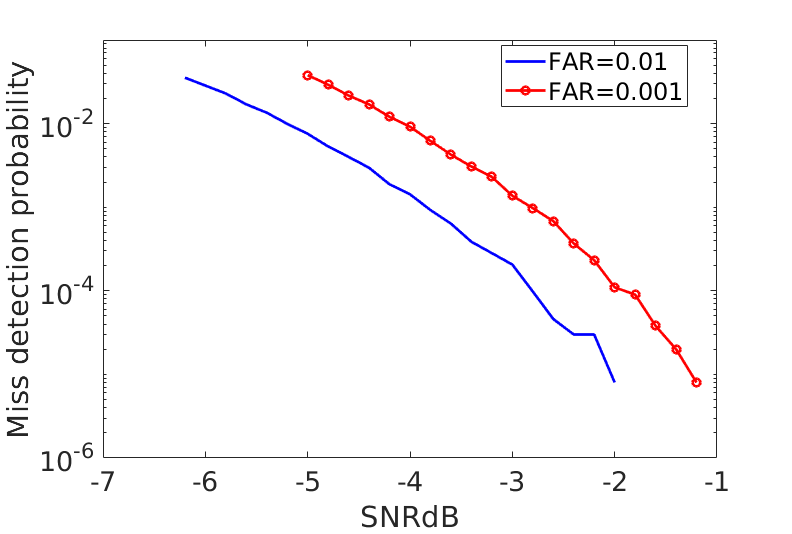
\includegraphics[scale=0.22]{fig2.png}}
\caption{DMRS detection performance.}
\label{fig5}
\vspace{-3mm}
\end{figure}

Simulation parameters for the performance of DMRS detection of each repetition in Fig.~\ref{fig5} are shown in Table~\ref{tab2}. For each DMRS detection, the correlation result is compared with a threshold to determine whether DMRS exists or not. This threshold is chosen according to a target false alarm rate (FAR) indicating the cases that the gNB determines the existence of DMRS while in reality there is no DMRS transmitted. A higher threshold is required for a lower FAR but also results in more missed detection. As DMRS dectection is mandatory for channel estimation to decode data as well as for recognizing UE ID to reschedule a retransmission if necessary in conventional scheme, a degradation of DMRS detection due to a smaller number of repetitions than configured makes the system not be able to support reliability URLLC requirement.

\begin{table}[htbp]
\caption{Performance comparison of different schemes when data comes after the first occasion in a period at $SNR = -5dB$ and $FAR = 0.001$}
\begin{center}
\begin{tabular}{|p{6em}|p{3em}|p{3em}|p{3.2em}|p{3.2em}|p{3.2em}|}
 \hline
 \textbf{Case} & \textbf{Starting time offset (ms)}&\textbf{Number of repetitions}&\textbf{UE ID miss-detection probability}&\textbf{Retrans in ID miss-detection}&\textbf{Total UE ID miss-detection probability}\\
 \hline
 Conventional transmission&$0$&$3$&$5.5\times10\textsuperscript{-5}$&$0$&$5.5\times10\textsuperscript{-5}$\\
 \hline
 Conventional transmission with the UE waiting the next period&$0.75$&$1$&$0.038$&$0$&$0.038$\\
 \hline
Transmission with explicit ACK&$0$&$3$&$5.5\times10\textsuperscript{-5}$&$1$&$2.1\times10\textsuperscript{-6}$\\
\hline
Transmission with SR&$0$&$3$&$2.1\times10\textsuperscript{-6}$&$0$&$2.1\times10\textsuperscript{-6}$\\
 \hline
\end{tabular}
\label{tab3}
\end{center}
\vspace{-3mm}
\end{table}

\begin{table}[htbp]
\caption{Performance comparison of different schemes when data comes after the second occasion in a period at $SNR = -5dB$ and $FAR = 0.001$}
\begin{center}
\begin{tabular}{|p{6em}|p{3em}|p{3em}|p{3.2em}|p{3.2em}|p{3.2em}|}
 \hline
 \textbf{Case} & \textbf{Starting time offset (ms)}&\textbf{Number of repetitions}&\textbf{UE ID miss-detection probability}&\textbf{Retrans in ID miss-detection}&\textbf{Total UE ID miss-detection probability}\\
 \hline
 Conventional transmission&$0$&$2$&$10\textsuperscript{-3}$&$0$&$10\textsuperscript{-3}$\\
 \hline
 Conventional transmission with the UE waiting the next period&$0.5$&$2$&$10\textsuperscript{-3}$&$0$&$10\textsuperscript{-3}$\\
 \hline
Transmission with explicit ACK&$0$&$2$&$10\textsuperscript{-3}$&$2$&$2.1\times10\textsuperscript{-6}$\\
\hline
Transmission with SR&$0$&$2$&$5.5\times10\textsuperscript{-5}$&$0$&$5.5\times10\textsuperscript{-5}$\\
 \hline
\end{tabular}
\label{tab4}
\end{center}
\vspace{-3mm}
\end{table}

\begin{table}[htbp]
\caption{Performance comparison of different schemes when data comes after the third occasion in a period at $SNR = -5dB$ and $FAR = 0.001$}
\begin{center}
\begin{tabular}{|p{6em}|p{3em}|p{3em}|p{3.2em}|p{3.2em}|p{3.2em}|}
 \hline
 \textbf{Case} & \textbf{Starting time offset (ms)}&\textbf{Number of repetitions}&\textbf{UE ID miss-detection probability}&\textbf{Retrans in ID miss-detection}&\textbf{Total UE ID miss-detection probability}\\
 \hline
 Conventional transmission&$0$&$1$&$0.038$&$0$&$0.038$\\
 \hline
  Conventional transmission with the UE waiting the next period&$0.25$&$3$&$5.5\times10\textsuperscript{-5}$&$0$&$5.5\times10\textsuperscript{-5}$\\
 \hline
Transmission with explicit ACK&$0$&$1$&$0.038$&$3$&$2.1\times10\textsuperscript{-6}$\\
\hline
Transmission with SR&$0$&$1$&$10\textsuperscript{-3}$&$0$&$10\textsuperscript{-3}$\\
 \hline
\end{tabular}
\label{tab5}
\end{center}
\vspace{-7mm}
\end{table}

In considered system, periodicity $P$ of HARQ process is 4 slots spreading in 1ms with SCS of 60kHz. The UE is configured to transmit 4 repetitions. As specified in \cite{ad2}, each slot only contains one repetition so one repetition consumes 0.25ms and the UE needs 4 slots to carry out all 4 configured repetitions and satisfies URLLC latency budget of 1ms.

Table~\ref{tab3}, Table~\ref{tab4} and Table~\ref{tab5} show the performance of DMRS detection at SNR of -5dB and FAR of 0.001 in various schemes and arrival time of data. As can be seen with conventional  transmission, due to the constraint of boundary of a period $P$, the UE cannot transmit 4 configured repetitions and it affects DMRS detection's performance. The later the packet comes, the worse DMRS detection is. In the timer-based feedback of the conventional scheme, the packet is lost because the UE assumes a successful transmission in case of DMRS miss-dection. Even if the UE waits for the next period with the intention of carrying of K repetitions configured as the second scheme, it also cannot achieve that intention because of URLLC latency requirement of 1ms. The more time the UE waits, the less time it has to transmit the repetitions. In consequence, it also cannot transmit K repetitions and DMRS miss-detection grows.

The presence of explicit feedback solves the problem of an increase of DMRS-miss detection because it helps the UE differentiate between a successful transmission and DMRS-miss detection. Therefore, the UE is able to retransmit packet even if the gNB does not detect UE ID by DMRS detection and reliability is guaranteed (total miss-detection probability of $2.1\times10\textsuperscript{-6}$ smaller than the conventional schemes) as shown in Table~\ref{tab3}, Table~\ref{tab4} and Table~\ref{tab5}.

These three tables also show that an additional SR transmitted in parallel with data provides another chance for the gNB to identify the UE and compensates for the missing repetitions due to boundary constraint so system performance is enhanced. 

The usages of an explicit feedback or an additional SR increase resource consumption. However, these approaches are only used in the critical situation as less than K repetitions made by the UE so a growth of resource consumption is limited. In addition, in case of less than K repetitions, the URLLC performance is degraded. Regarding the priorities of latency and reliability, resources used for the explicit feedback or the SR are necessary to guarantee those strict requirements.

\section{Conclusion}\label{V}

In URLLC GF UL transmission. a packet is configured with K repetitions to achieve target QoS. However, because of boundary of a period P and arrival time of data, the UEs are only able to transmit less than K repetitions so the target QoS is not attained. This paper presents two strategies to help the UEs achieve the target QoS in case of less than K repetitions. These approaches relating to an explicit HARQ strucutre and an additional SR can be used individually or combined together based different scenarios. The results show that they improve the UE ID detection at the gNB.

\begin{thebibliography}{00}
\bibitem{b6} 3GPP TR 38.913 v15.0.0, ``Study on scenarios and requirements for next generation access technologies.''
\bibitem{b8} Huawei, HiSilicon, Nokia, Nokia Shanghai Bell, ``New SID on Physical Layer Enhancements for NR URLLC''. 3GPP RP-182089, TSG-RAN\#81, Gold Coast, Australia, Sept 10--13, 2018.
\bibitem{ad2} 3GPP TS 38.211 v15.3.0, ``Physical channels and modulation.''
\bibitem{ad3} 3GPP TR 38.802 v14.2.0, ``Study on new radio access technology physical layer aspects.''
\bibitem{ad4} 3GPP TS 38.214 v15.3.0, ``Physical layer procedures for data.''
\bibitem{ad5} 3GPP TS 38.331 v15.3.0, ``Radio Resource Control (RRC) protocol specification.''
\bibitem{b1} Ericsson, ``Enhancement of Configured Grant for NR URLLC'', 3GPP R1-1812162, RAN1\#95, Spokane, USA, November 12--16, 2018.
\bibitem{b2} Huawei, HiSilicon, ``Enhanced UL configured grant transmissions'', 3GPP R1-1812226, RAN1\#95, Spokane, USA, November 12--16, 2018.
\bibitem{b3} Intel Corporation, ``On enhanced Configured Grant PUSCH for eURLLC'', 3GPP R1-1812506, RAN1\#95, Spokane, USA, November 12--16, 2018.
\bibitem{b4} Sony, ``Discussion on enhanced UL grant-free transmissions'', 3GPP R1-1812746, RAN1\#95, Spokane, USA, November 12--16, 2018.
\bibitem{b5} R. breu, G. Berardinelli, T. Jacobsen, K. Pedersen and P. Mogensen, ``A Blind Retransmission Scheme for Ultra-Reliable and Low Latency Communications'', 2018 IEEE 87th Vehicular Technology Conference (VTC Spring), June 2018.
\bibitem{b7} Z. Zhou, R. Ratasuk, N. Mangalvedhe and A. Ghosh, ``Resource Allocation for Uplink Grant-Free Ultra-Reliable and Low Latency Communications'', 2018 IEEE 87th Vehicular Technology Conference (VTC Spring), June 2018.
%\bibitem{b9} B. Singh, O. Tirkkonen, Z. Li and M. A. Uusitalo, ``Contention-Based Access for Ultra-Reliable Low Latency Uplink Transmissions'',  IEEE Wireless Communications Letters, April 2018.

\end{thebibliography}
\vspace{12pt}


\end{document}
